\chapter{Conclusions}
\label{conclusion}

In this thesis we described the quantum-mechanical phenomenon of \textit{backflow} in the non-interacting and interacting scenario, using methods from operator theory. In particular, we outlined the fundamental properties of backflow effect and its magnitude in different frameworks.\\
In Chapter 2, we gave the definition of backflow for free particles introducing the concept of \textit{right-movers} as those wave-functions with only positive momenta and we outlined some examples of right-moving wave-functions in which backflow occurs. Then, we showed that the lower bound in the amount of probability which might "flow backwards" is equivalent to the infimum of the spectrum of a suitable operator $B$, called \textit{backflow operator}. Since $B$ is bounded and self-adjoint, this lower bound $\lambda$ exists. At the end of the chapter, we used  numerical methods to evaluate $\lambda$, obtaining $\lambda\approx0.038452$.\\
In Chapter 3, we extended the analysis of backflow to an interacting system. In particular, we considered particles scattering with a short-range potential $V$ and we investigated the existence of backflow in this framework. We reformulated the problem of backflow by defining \textit{asymptotic right-movers}, as those wave-functions that, far from the potential, behave like free right-movers. We observed that each interaction-free right-mover $\psi$ is the incoming asymptote of an interacting state $\Omega_V\psi$, where $\Omega_V$ is the \textit{M\o{}ller operator} of the Hamiltonian with potential $V$. Then we analyzed the spatially averaged current
\begin{equation*}
	\int_{-\infty}^{\infty}\nspace\!f(x)j_{\Omega_V\psi}(x)\,\dd x\,,
\end{equation*}
with $\Omega_V\psi$ representing the interacting wave-function. To prove that this integral assumes negative values for suitable positive $f\ge0$, we needed to evaluate the infimum of the spectrum of a proper \textit{asymptotic current operator}. In the end, we proved that there exists a lower bound on the backflow, i.e. for all short-range potential $V$ and smearing positive functions $f\ge0$, there exists a constant $\beta_V(f)\in(-\infty,0)$ such that the spatially averaged backflow is always larger than $\beta_V(f)$. The existence of backflow might not seem surprising in presence of a potential, because the reflection component of any incoming wave yields a probability flow to the left. Yet our results also holds even for potentials lacking such reflection.\\
\\
\\
The possible extensions and follow-ups of this work are manifold. Firstly, numerical methods can be used to estimate the constant $\beta_V(f)$ for different averaging functions $f$ and potentials $V$. In [\citealp[Sect. IV]{gand}], this analysis is made by considering a Gaussian function for $f$ and a \textit{Delta potential} $V(x)=\alpha\delta(x)$ as well as the reflection-less \textit{P\"{o}schl-Teller potential}
\begin{equation*}
	V(x)=-\frac{\mu(\mu+1)}{2\cosh^2(x)}\ \ \text{with}\ \mu\in\mathbb{N}\,.
\end{equation*}
Secondly, we remark that backflow has been studied only theoretically and no experimental observations has been conducted. The weakness of backflow represents a remarkably issue for any experimental set-up that tries to measure this quantum effect. A possible experimental scheme that could lead to the first observation
of quantum backflow is made by Palmero \textit{et al.} in [\citealp{palmero}]. They suggest to use Bose-Einstein condensates. In detail, the application of a positive momentum kick, via a Bragg pulse\footnote{For a more detailed discussion on the Bragg pulse, see [\citealp{bragg}]}, to such a condensate with
a positive velocity may cause a current flow in the negative direction. A sketch of the experimental set-up, as in Figure \ref{fig:bose}, is the following:
\begin{figure}[h!]
	\centering
	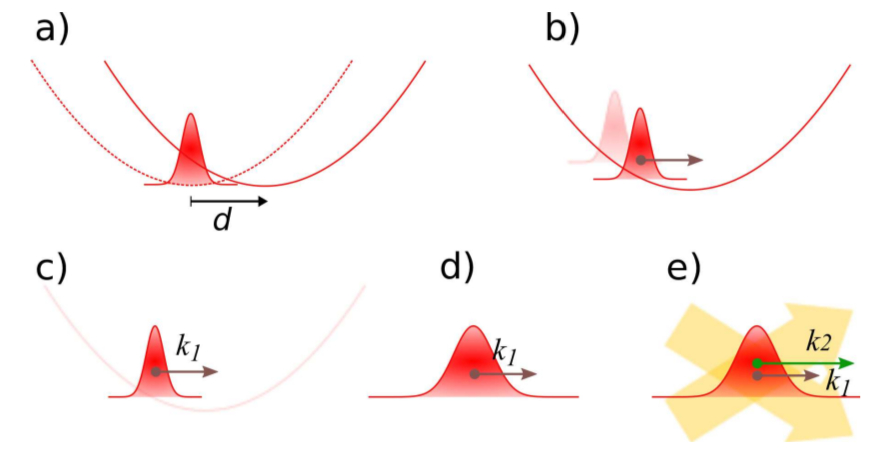
\includegraphics[scale=0.30]{images/bose}
	\caption{Sketch of the experimental set-up proposed in [\citealp{palmero}]}
	\label{fig:bose}
\end{figure}
\begin{itemize}
	\item[(a)] A condensate is created in the
	ground state of a harmonic trap with frequency $\omega$ ; at $t = 0$
	a magnetic gradient is applied, shifting the trap by a distance
	$d$.
	\item[(b)]The condensate starts to perform dipole oscillations in
	the trap.
	\item[(c)]When the condensate reaches a desired momentum $k_1$, the trap
	is switched off.
	\item[(d)]The condensate is let to expand for an interval of time $t$.
	\item[(e)]Finally, a Bragg pulse is applied in order to transfer part of the to a state of momentum $k_2$. The superposition of states with momentum $k_1$ and $k_2>k_1$ causes backflow.
\end{itemize}
